\documentclass[12pt]{report}
\setlength{\parskip}{1em}
\parindent0mm
\textwidth150mm
\textheight200mm
\oddsidemargin+5mm

\usepackage[pdftex]{graphicx}
\usepackage{color}
\usepackage{amsfonts}
\usepackage{longtable}
\usepackage{hyperref}			  % Custom hyperlinks

% Setup hyperlink format in document
\hypersetup{
    colorlinks=true, %set true if you want colored links
    linkcolor=blue,  %choose some color if you want links to stand out
    citecolor=blue,  %choose some color if you want lcitation to stand out
    filecolor=black, % etc...
    urlcolor=blue
}

\definecolor{LightBlue}{rgb}{0.8,0.85,1}
\definecolor{LightGrey}{gray}{.85}
\setlength{\fboxrule}{1pt}
\setlength{\fboxsep}{2pt}
\setlongtables

\newcommand{\vect}[1]{\ensuremath{\mathrm{\mathbf{#1}}}}
\newcommand{\pdiv}[2]{\ensuremath{\frac{\partial #1}{\partial #2}}}
\newcommand{\WarningBox}[1]{
  %\fcolorbox[rgb]{0,0,0}{0.95,0.95,0.95}{
    \fcolorbox{black}{LightGrey}{
    \begin{minipage}{0.965\linewidth}
      \textbf{WARNING:}
      #1
    \end{minipage}
  }
}

\begin{document}

%Cover page
\thispagestyle{empty}	%don't include number on cover
%\begin{flushleft}
%\begin{figure}
%
\includegraphics[width=0.2\textwidth]{gplv3-127x51.png}
%\end{figure}
%\end{flushleft}
\verb+ +
\vspace{1em}
\begin{flushright}
\huge\bf MP-LABS v1.6\\
\rule{\textwidth}{4pt}
\large{\bf MultiPhase Lattice Boltzmann Suite User Guide\\
Document Revision 1.0\\
\today}
\end{flushright}

\vspace{1cm}
\begin{figure}[!hbt]
\centering
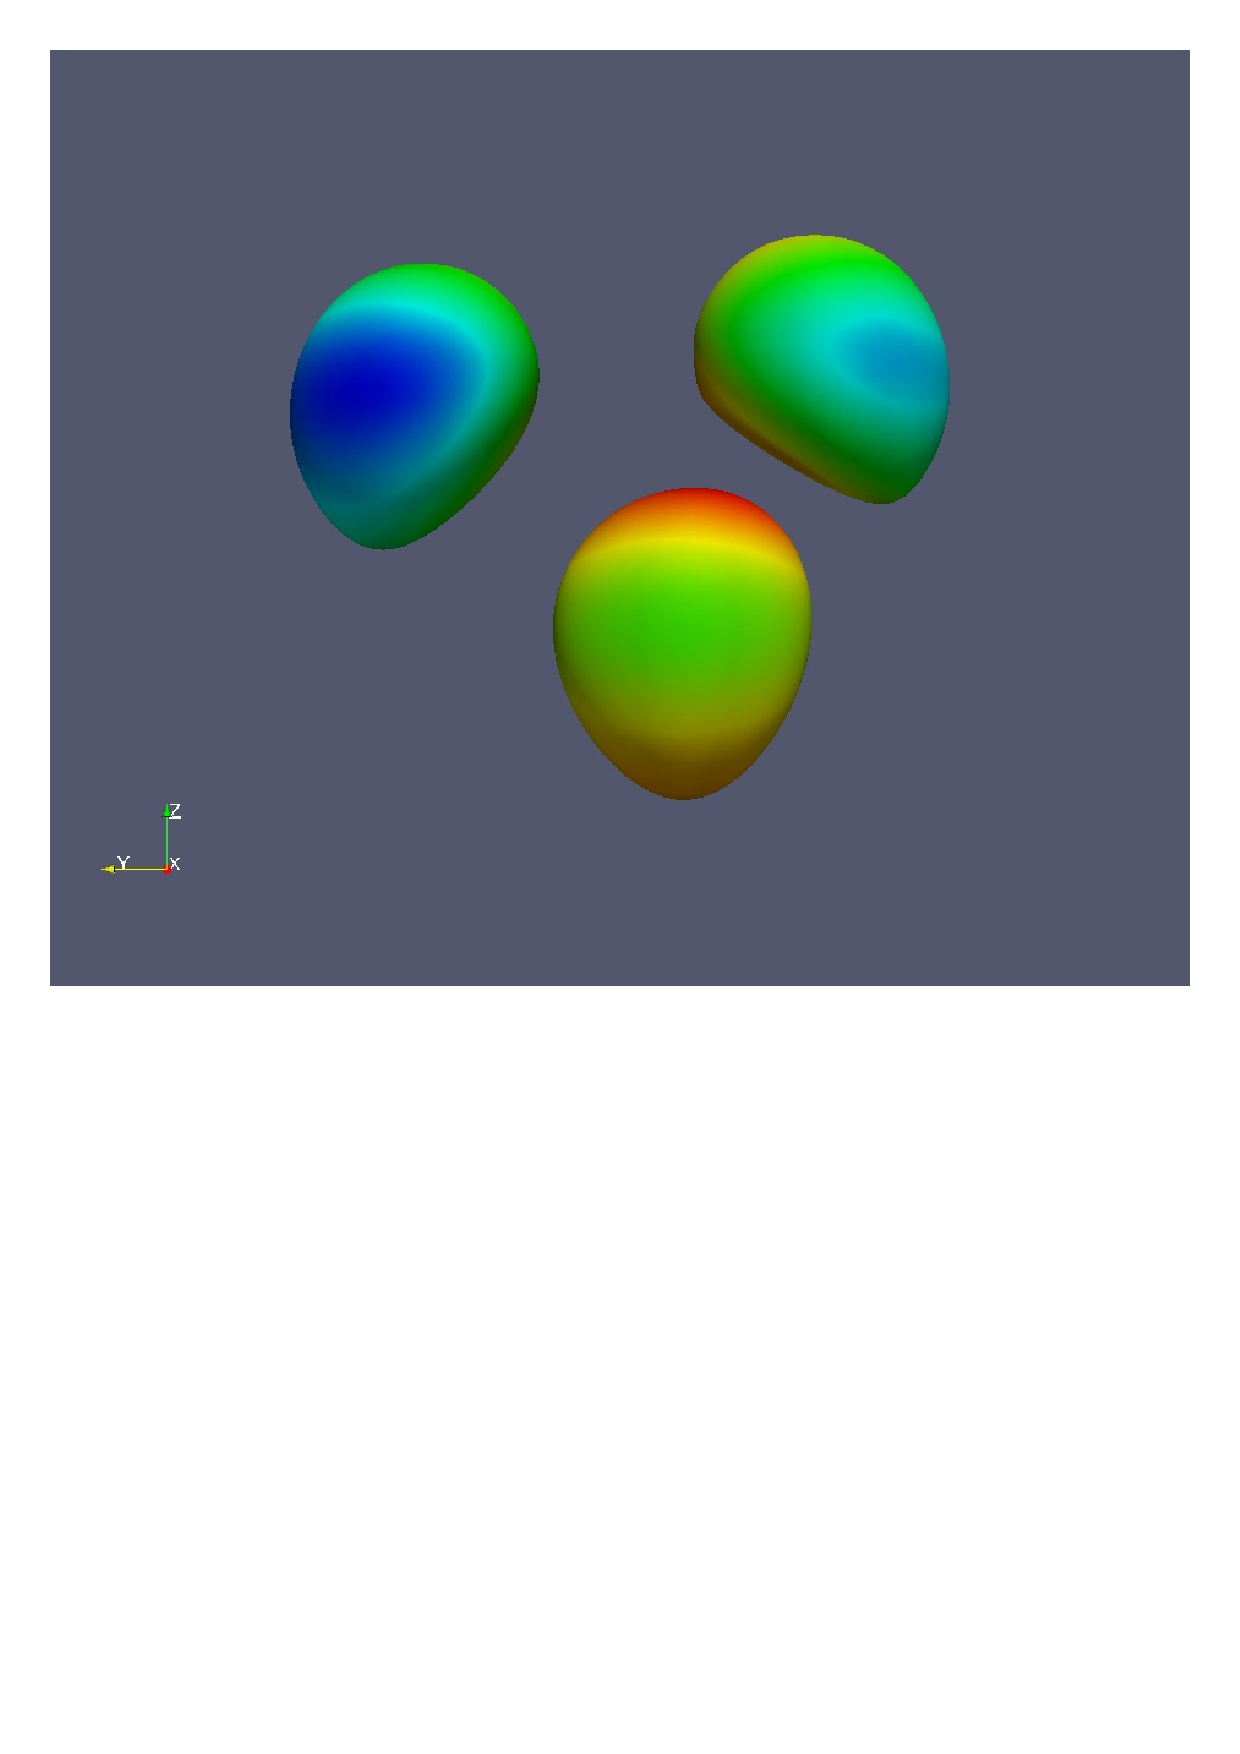
\includegraphics[width=0.5\textwidth]{bubble_3.pdf}
\end{figure}

%Back of cover page (copyright)
\newpage
\thispagestyle{empty}
\begin{flushleft}
\begin{figure}

\includegraphics[width=0.2\textwidth]{gplv3-127x51.png}
\end{figure}
Carlos Rosales Fern\'andez\\
\verb+carlos@tacc.utexas.edu+\\
\vspace{0.5em}
High Performance Computing \\
Texas Advanced Computing Center\\
The University of Texas at Austin\\
\vspace{1cm}
Copyright \copyright 2014 Carlos Rosales Fern\'andez and the University of Texas at Austin.
\end{flushleft}
\newpage


\pagenumbering{roman}	%for preface sections only
\section*{Preface}\noindent \verb+MP-LABS+ is a suite of numerical simulation tools for multiphase flows based on the free energy Lattice Boltzmann Method (LBM). The code allows for the simulation of quasi-incompressible two-phase flows, and uses multiphase models that allow for large density ratios. \verb+MP-LABS+ provides implementations that use periodic boundary conditions, but it is written in a way that allows for easy inclusion of different boundary conditions. The output from \verb+MP-LABS+ is in plain ASCII and VTK format, and can be analyzed using other Open Source tools such as Gnuplot \cite{gnuplot} and Paraview \cite{paraview}.

\noindent Revision 1.6 adds a simplified build system that makes easier to build Xeon Phi executables.

\noindent The objective of the \verb+MP-LABS+ project is to provide a core set of routines that are well documented, highly portable, and have proven to perform well in a variety of systems. The source code is written in Fortran 90, OpenMP  and MPI and uses separate subroutines for most tasks in order to make modifications easier. An examples of research work performed using this code are references \cite{Rosales2007} and \cite{Rosales2010}.

\noindent We believe in open source software for pushing the frontiers of science and engineering, and we encourage everyone to publish open source software under the GPL License. You are free to use, copy, modify and distribute any element of \verb+MP-LABS+ under the GNU General Public License version 3. Finally, although the GPL License does not require you to contact us, the authors would appreciate if you could send an email telling us that you are using \verb+MP-LABS+ and what application you are using the code for.

\noindent The complete package can be downloaded from \verb+github.com/carlosrosales/mplabs+.

\vspace{1cm}
	Carlos Rosales Fern\'andez\\
	\today

\pagebreak
\section*{}
\pagebreak

\tableofcontents
\pagebreak
\section*{}
\pagebreak

\pagenumbering{arabic}	%for preface sections only

\chapter{Installation}
\verb+MP-LABS+ is distributed as a series of Fortran 90 subroutine files, and a series of Make files. The complete list of functions is collected in Appendix A.

\section{Quick Install}
Download \verb+mplabs-1.6.tar.gz+ from \verb+github.com/carlosrosales/mplabs+. Unzip the \verb+mplabs-1.6.tar.gz+ file in a suitable directory:

\begin{tabular}{l}
\texttt{\$ tar -zxvf mplabs-1.6.tar.gz}
\end{tabular}

Once the file has been unpackaged move into the \verb+mplabs+ directory and type:

\begin{tabular}{l}
\texttt{\$ make \&\& make install}
\end{tabular}

The compilation uses by default GNU's gfortran for the serial code and the wrapper mpif90 for the parallel code, with the flag -O3. If for some reason you don't like this, or you would like to add an architecture-related flag read Section \ref{sec:compilation} for details. 

Assuming you meet all the installation requirements, the binary files are now in the directory \verb+mplabs/bin+ and the documentation is in \verb+mplabs/docs+. Enjoy!


\section{Installation}
Download \verb+mplabs-1.6.tar.gz+ from \verb+github.com/carlosrosales/mplabs+. Unzip the \verb+mplabs-1.6.tar.gz+ file in a suitable directory. This can be done in a linux system by typing on the command line:

\begin{tabular}{l}
\texttt{\$ tar -zxvf mplabs-1.6.tar.gz}
\end{tabular}

or, if tar does not accept the "z" option in your system:

\begin{tabular}{l}
\texttt{\$ gunzip mplabs-1.6.tar.gz}\\
\texttt{\$ tar -xvf mplabs-1.6.tar}
\end{tabular}

The following directories will be created:

\begin{tabular}{ll}
\texttt{mplabs}&: Main program directory, license and readme files\\
\texttt{mplabs/bin}&: Binary files are stored here after compilation\\
\texttt{mplabs/docs}&: Code documentation\\
\texttt{mplabs/examples}&: Examples to test the installation\\
\texttt{mplabs/src}&: Fortran 90 source code\\
\texttt{mplabs/src/devel}&: Source code for development implementations\\
\texttt{mplabs/src/opt}&: Source code for optimized implementations\\
\texttt{mplabs/src/std}&: Source code for standard implementations\\
\end{tabular}

\subsection{Requirements}
In order to install and run \verb+MP-LABS+ all the \verb+.F90+ files listed in Appendix A are necessary. Make sure the uncompressed files exist in their corresponding directories within \verb+mplabs/src+.

Besides the source code for \verb+MP-LABS+ you will also need working versions of:

\begin{itemize}
\item A Fortran compiler such as gfortran,
\item Make,
\item An MPI library such as OpenMPI \cite{openmpi} (only for the parallel version).
\end{itemize}

\subsection{Compilation}
\label{sec:compilation}
A total of ten executables can be compiled in \verb+MP-LABS+. The first eight executables correspond to 2D serial and parallel (MPI) versions of standard and dual grid implementations of the Zheng-Shu-Chew multiphase LBM \cite{Zheng2006} and the Lee-Lin multiphase LBM \cite{Lee2005}. The ninth version is the 3D implementation of the Zheng-Shu-Chew multiphase LBM. The tenth binary is an optimized version of the later. For ease of reference in the rest of this document the two models will be called ZSC-LBM and LL-LBM. The name codes of the executables are self-explanatory, and the following table can be used as a reference (source code directories are within \texttt{mplabs/src/}):

\begin{tabular}{|l|l|c|c|c|c|l|}
\hline
Name & Model & Type & OMP & MPI & Dual Grid & Source Dir\\
\hline
\texttt{LL-2D-DGR}& Lee \& Lin & D2Q9 & &   & * & \texttt{std/ll-dgr-seq}\\
\hline
\texttt{LL-2D}& Lee \& Lin & D2Q9 &   & &   & \texttt{std/ll-seq}\\
\hline
\texttt{LL-2D-DGR-MPI}& Lee \& Lin & D2Q9 & & * & * & \texttt{std/ll-dgr-mpi}\\
\hline
\texttt{LL-2D-MPI}& Lee \& Lin & D2Q9 & & * &   & \texttt{std/ll-mpi}\\
\hline
\texttt{ZSC-2D-DGR}& Zheng \it{et al} & D2Q9 & &   & * & \texttt{std/zsc-dgr-seq}\\
\hline
\texttt{ZSC-2D}& Zheng \it{et al} & D2Q9 & &   &   & \texttt{std/zsc-seq}\\
\hline
\texttt{ZSC-2D-DGR-MPI}& Zheng \it{et al} & D2Q9 &  & * & * & \texttt{std/zsc-dgr-mpi}\\
\hline
\texttt{ZSC-2D-MPI}& Zheng \it{et al} & D2Q9 & & * &   & \texttt{std/zsc-mpi}\\
\hline
\texttt{ZSC-3D-MPI}& Zheng \it{et al} & D3Q19 & & * &   & \texttt{std/zsc-3d-mpi}\\
\hline
\texttt{LBS3D}& Zheng \it{et al} & D3Q19 & * &  &   & \texttt{opt/lbs3d}\\
\hline
\texttt{LBS3D-MPI}& Zheng \it{et al} & D3Q19 & * & * &   & \texttt{opt/lbs3d-mpi}\\
\hline
\end{tabular}

In addition to the baseline codes in \texttt{mplabs/src/std} and \texttt{mplabs/src/opt} a number of intermediate development codes have been provided to illustrate the process of improving performance of a code, starting from a na\"ive serial implementation and progressing to a code equivalent to LBS3D. These codes follow the Zheng \textit{et al} 3D model, and are located in the \texttt{mplabs/src/devel} directory. An example of offload execution to the Intel Xeon Phi while also using the host CPU is provided. The following table provides additional details:

 \begin{tabular}{|l|c|c|l|}
\hline
Name & OMP & Offload & Source Dir\\
\hline
\texttt{LBS3D-DEVEL-SEQ}&  &  & \texttt{devel/sequential}\\
\hline
\texttt{LBS3D-DEVEL-OMPv1}& Collision Only &  & \texttt{devel/omp\_v1}\\
\hline
\texttt{LBS3D-DEVEL-OMPv2}& * &  & \texttt{devel/omp\_v2}\\
\hline
\texttt{LBS3D-DEVEL-SOA}& * &  & \texttt{devel/soa}\\
\hline
\texttt{LBS3D-DEVEL-SOA\_AL}& * &  & \texttt{devel/soa\_aligned}\\
\hline
\texttt{LBS3D-DEVEL-OFFLOAD}& * & * & \texttt{devel/offload}\\
\hline
\end{tabular}

Edit the \verb+mplabs/Makefile.in+ file in order to define the compiler, compiler options, and installation directory. This is the only file where you should have to make changes in order to build the software.

The provided Makefile can be used to build the sequential codes only:

\begin{tabular}{l}
\texttt{\$ make seq}\\
\texttt{\$ make seq-install}
\end{tabular}

The MPI parallel codes only:

\begin{tabular}{l}
\texttt{\$ make par}\\
\texttt{\$ make par-install}
\end{tabular}

The optimized code only:

\begin{tabular}{l}
\texttt{\$ make opt}\\
\texttt{\$ make opt-install}
\end{tabular}

or everything:

\begin{tabular}{l}
\texttt{\$ make }\\
\texttt{\$ make install}
\end{tabular}

The development codes must be built and installed separately:

\begin{tabular}{l}
\texttt{\$ make devel}\\
\texttt{\$ make devel-install}
\end{tabular}

This will compile the relevant source code and move the binary files to \verb+INSTALL_DIR/bin+, with the \verb+INSTALL_DIR+ defined in Makefile.in.

\subsection{Multiple Versions}
Use the provided variable \verb+BIN_SUFFIX+ in order to add an informative suffix to your binary files. This could be an indication of the compiler flags used such as \verb+.dbg+ or \verb+.opt+, or an indication of the architecture such as \verb+.cpu+ or \verb+.mic+.

This variable can be defined in the command line when invoking Make, exported tot he environment, or defined in \verb+Makefile.in+. The definition in Makefile.in will take precedence.

\subsection{Building the optimized Xeon Phi Version}
A simple way to build a Xeon Phi compatible version is provided. Use the following options to generate both host CPU and Xeon Phi versions of the \verb+LBS3D+ code:

\begin{tabular}{l}
\texttt{\$ make opt compiler=intel build=cpu suffix=.cpu}\\
\texttt{\$ make opt-install compiler=intel build=cpu suffix=.cpu}\\
\texttt{\$ make clean}\\
\texttt{\$ make opt compiler=intel build=mic suffix=.mic}\\
\texttt{\$ make opt-install compiler=intel build=mic suffix=.mic}
\end{tabular}

An example appropriate for running a symmetric execution that uses 3 total MPI tasks (suggested configuration is 2 MPI tasks on the Phi coprocessor and 1 task on the host CPU) is provided under \verb+/examples/opt/lbs3d-symmetric+.

\chapter{Input Files}
There are two input files required to run any simulation, one called \verb+properties.in+ which contains all the simulation parameters, and another one called \verb+discrete.in+ which contains a description of the discrete phase.

The input file format is identical for standard and dual grid implementations, but slightly different for the Lee-Lin and Zheng-Shu-Chew versions as they require different parameters. This chapter describes the input files in detail.

\section{Lee-Lin Properties File}
The properties file \verb+properties.in+ for the Lee-Lin model contains the following variables:

\begin{longtable}{rl}
\textit{MaxStep}  :& Maximum number of iterations to run.\\
\textit{tStat}    :& Iterations between statistical data writes to \verb+stats.out+.\\
\textit{tDump}    :& Iterations between hydrodynamics data writes to VTK files.\\
\textit{xmin}     :& Minimum x value in the geometry.\\
\textit{xmax}     :& Maximum x value in the geometry.\\
\textit{ymin}     :& Minimum y value in the geometry.\\
\textit{ymax}     :& Maximum y value in the geometry.\\
\textit{rhoL}     :& Density of the lighter fluid.\\
\textit{rhoH}     :& Density of the heavier fluid.\\
\textit{tauL}     :& Relaxation time for the lighter fluid.\\
\textit{tauH}     :& Relaxation time for the heavier fluid.\\
\textit{IntWidth} :& Interface width in lattice units.\\
\textit{sigma}    :& Interfacial tension.\\
\textit{pConv}    :& Maximum relative error for pressure convergence.\\
\textit{mpi\_xdim}:& [OPT: MPI only] Number of partitions in x.\\
\textit{mpi\_ydim}:& [OPT: MPI only] Number of partitions in y.\\
\end{longtable}

This file typically takes the following form:

\fcolorbox{black}{LightBlue}{
\begin{tabular}{l}
\texttt{MaxStep}\\
\texttt{50000}\\
\texttt{tStat, tDump}\\
\texttt{100,   2000}\\
\texttt{xmin, xmax, ymin, ymax}\\
\texttt{1,    300,  1,    100}\\
\texttt{rhoL,    rhoH}\\
\texttt{0.001D0, 1.D0}\\
\texttt{tauL,  tauH}\\
\texttt{1.0D0, 0.1D0}\\
\texttt{IntWidth, sigma}\\
\texttt{5.0D0,    0.001D0}\\
\texttt{pConv}\\
\texttt{0.001D0}\\
\texttt{mpi\_xdim, mpi\_ydim}\\
\texttt{1,        2}\\
\end{tabular}
}

where the last two lines are only required for the parallel versions of the code, and will be ignored by the serial code.

If this input file is provided a regular cartesian grid of size $300\times100$ will be used for the simulation, which will run for a maximum of 50000 iterations or until the relative pressure error is below \verb+pConv+ = 0.001.

The average velocity of the discrete phase, the mas conservation factor, the effective bubble radius, the pressure difference between the interior of the bubble and the continuous phase, and the error with respect to Laplace's Law ($P_{\rm in} - P_{rm out} = \sigma/R$) will be saved to the file \verb+stats.out+ every 100 iterations.

The order parameter, pressure and velocity values for the full computational domain will be saved in VTK format every 2000 iterations to files DATA\_0002000.vtk, DATA\_0004000.vtk, etc...

Notice that for the parallel cases the total number of processors used is given by the product \texttt{nprocs = mpi\_xdim$\times$mpi\_ydim} and not by the sum.


\section{Zheng-Shu-Chew Properties File}
The properties file \verb+properties.in+ for the Zheng-Shu-Chew model contains the following variables:

\begin{longtable}{rl}
\textit{MaxStep}  :& Maximum number of iterations to run.\\
\textit{RelaxStep}:& [OPT: 3D only] Maximum number of steps in the relaxation run.\\
\textit{tStat}    :& Iterations between statistical data writes to \verb+stats.out+.\\
\textit{tDump}    :& Iterations between hydrodynamics data writes to VTK files.\\
\textit{xjump}    :& [OPT: 3D Only] Save every {\it xjump} nodes to the VTK otuput files.\\ 
\textit{xmin}     :& Minimum x value in the geometry.\\
\textit{xmax}     :& Maximum x value in the geometry.\\
\textit{ymin}     :& Minimum y value in the geometry.\\
\textit{ymax}     :& Maximum y value in the geometry.\\
\textit{zmin}     :& [OPT: 3D only] Minimum z value in the geometry.\\
\textit{zmax}     :& [OPT: 3D only] Maximum z value in the geometry.\\
\textit{rhoL}     :& Density of the lighter fluid.\\
\textit{rhoH}     :& Density of the heavier fluid.\\
\textit{tauRho}   :& Relaxation time.\\
\textit{tauPhi}   :& Relaxation parameter for the phase.\\
\textit{IntWidth} :& Interface width in lattice units.\\
\textit{sigma}    :& Interfacial tension.\\
\textit{Gamma}    :& Interface mobility.\\
\textit{pConv}    :& Maximum relative error for pressure convergence.\\
\textit{mpi\_xdim} :& [OPT: MPI only] Number of partitions in x.\\
\textit{mpi\_ydim} :& [OPT: MPI only] Number of partitions in y.\\
\textit{mpi\_zdim} :& [OPT: 3D MPI only] Number of partitions in z.\\
\end{longtable}

This file typically takes the following form for a 2D simulation:

\fcolorbox{black}{LightBlue}{
\begin{tabular}{l}
\texttt{MaxStep}\\
\texttt{50000}\\
\texttt{tStat, tDump}\\
\texttt{100,   2000}\\
\texttt{xmin, xmax, ymin, ymax}\\
\texttt{1,    300,  1,    100}\\
\texttt{rhoL,  rhoH}\\
\texttt{1.0D0, 1000.D0}\\
\texttt{tauRho,  tauPhi}\\
\texttt{0.6D0, 0.7D0}\\
\texttt{IntWidth, sigma,  Gamma}\\
\texttt{5.0D0,    0.01D0, 200.D0}\\
\texttt{pConv}\\
\texttt{0.001D0}\\
\texttt{mpi\_xdim, mpi\_ydim}\\
\texttt{1,        2}\\
\end{tabular}
}

where the last two lines are only required for the parallel versions of the code, and will be ignored by the serial code.

If this input file is provided a regular cartesian grid of size $300\times100$ will be used for the simulation, which will run for a maximum of 50000 iterations or until the relative pressure error is below \verb+pConv+ = 0.001.

The average velocity of the discrete phase, the mas conservation factor, the effective bubble radius, the pressure difference between the interior of the bubble and the continuous phase, and the error with respect to Laplace's Law ($P_{\rm in} - P_{rm out} = \sigma/R$) will be saved to the file \verb+stats.out+ every 100 iterations.

The order parameter, pressure and velocity values for the full computational domain will be saved in VTK format every 2000 iterations to files DATA\_0002000.vtk, DATA\_0004000.vtk, etc...

Notice that for the parallel cases the total number of processors used is given by the product \texttt{nprocs = mpi\_xdim$\times$mpi\_ydim} and not by the sum.

\section{LBS3D Properties File}
The properties file \verb+properties.in+ for the optimized code contains the following variables:

\begin{longtable}{rl}
\textit{MaxStep}  :& Maximum number of iterations to run.\\
\textit{RelaxStep}:& Maximum number of steps in the relaxation run.\\
\textit{tStat}    :& Iterations between statistical data writes to \verb+stats.out+.\\
\textit{tSave}    :& Iterations between hydrodynamics data writes to VTK files.\\
\textit{xmin}     :& Minimum x value in the geometry.\\
\textit{xmax}     :& Maximum x value in the geometry.\\
\textit{ymin}     :& Minimum y value in the geometry.\\
\textit{ymax}     :& Maximum y value in the geometry.\\
\textit{zmin}     :& Minimum z value in the geometry.\\
\textit{zmax}     :& Maximum z value in the geometry.\\
\textit{rhoL}     :& Density of the lighter fluid.\\
\textit{rhoH}     :& Density of the heavier fluid.\\
\textit{tauRho}   :& Relaxation time.\\
\textit{tauPhi}   :& Relaxation parameter for the phase.\\
\textit{IntWidth} :& Interface width in lattice units.\\
\textit{sigma}    :& Interfacial tension.\\
\textit{Gamma}    :& Interface mobility.\\
\textit{Eo}       :& Eotvos number, used to determine external gravity force.\\
\textit{pConv}    :& Maximum relative error for pressure convergence.\\
\textit{mpi\_xdim} :& [OPT: MPI only] Number of partitions in x.\\
\textit{mpi\_ydim} :& [OPT: MPI only] Number of partitions in y.\\
\textit{mpi\_zdim} :& [OPT: MPI only] Number of partitions in z.\\
\end{longtable}

This file typically takes the following form:

\fcolorbox{black}{LightBlue}{
\begin{tabular}{l}
\texttt{MaxStep, RelaxStep}\\
\texttt{50000, 1000}\\
\texttt{tStat, tSave}\\
\texttt{100,   2000}\\
\texttt{xmin, xmax, ymin, ymax, zmin, zmax}\\
\texttt{1,    300,  1,    100,  1,    100}\\
\texttt{rhoL,  rhoH}\\
\texttt{1.0D0, 1000.D0}\\
\texttt{tauRho,  tauPhi}\\
\texttt{0.6D0, 0.7D0}\\
\texttt{IntWidth, sigma,  Gamma}\\
\texttt{5.0D0,    0.01D0, 200.D0}\\
\texttt{Eo,  pConv}\\
\texttt{1.D0, 0.001D0}\\
\texttt{mpi\_xdim, mpi\_ydim, mpi\_zdim}\\
\texttt{1,        1,         2}\\
\end{tabular}
}

where the last two lines are only required for the parallel versions of the code, and will be ignored by the serial code.

If this input file is provided a regular cartesian grid of size $300\times100\times100$ will be used for the simulation, which will run without application of the external force for a maximum of 1000 iterations or until the relative pressure error is below \verb+pConv+ = 0.001. This relaxation loop is designed to relax the domain and minimize spurious velocities at the fluid-fluid interface before starting the 50000 step evolution loop that includes external forcing. 

The average velocity of the discrete phase, the mas conservation factor, the effective bubble radius, the pressure difference between the interior of the bubble and the continuous phase, and the error with respect to Laplace's Law ($P_{\rm in} - P_{rm out} = \sigma/R$) will be saved to the file \verb+stats.out+ every 100 iterations.

The order parameter, pressure and velocity values for the full computational domain will be saved in VTK format every 2000 iterations to files EVOL\_0002000.vtk, EVOL\_0004000.vtk, etc...

\section{Discrete Phase File}
The discrete phase file \verb+discrete.in+ contains the following variables:

\begin{longtable}{rl}
\textit{DISTRO}       :& [OPT: 3D only] Random (==1) or given (/=1) bubble positions.\\
\textit{xb}           :& [OPT: 3D, DISTRO=1 only] Number of different positions in x\\
\textit{yb}           :& [OPT: 3D, DISTRO=1 only] Number of different positions in y\\
\textit{zb}           :& [OPT: 3D, DISTRO=1 only] Number of different positions in z\\
\textit{rb}           :& [OPT: 3D, DISTRO=1 only] Radius of the bubbles.\\
\textit{nBubbles}     :& Number of bubbles to include.\\
\textit{bubbles(i,1)} :& x coordinate of the i{\it th} bubble.\\
\textit{bubbles(i,2)} :& y coordinate of the i{\it th} bubble.\\
\textit{bubbles(i,3)} :& radius of the i{\it th} bubble.\\
\end{longtable}

This file typically takes the following form for a 2D simulation:

\fcolorbox{black}{LightBlue}{
\begin{tabular}{l}
\texttt{nBubbles}\\
\texttt{2}\\
\texttt{xi, yi, ri}\\
\texttt{40, 51, 20}\\
\texttt{120, 51, 30}\\
\end{tabular}
}

This example will generate two bubbles, the first at $(40,51)$ with radius 20 lattice units, and the second at $(120,51)$ with radius 30 lattice units.

\WarningBox{
There is no limit to the number of bubbles/drops that can be included in the simulation, but one should be aware that the code does not check for overlap. Overlapping bubbles will be initialized as if they had merged and may produce unexpected simulation results.
}

\chapter{Multiphase Models}
This chapter describes the two multphase models available in \verb+MP-LABS+. In both cases the physical equations that are simulated are the Navier-Stokes equation together, the mass conservation equation, and a convective Cahn-Hilliard equation to track the interface evolution:

\begin{eqnarray}
  &&\pdiv{\rho}{t} + \vect{\nabla}\cdot(\rho\vect{u}) = 0,\label{eqn:mass_conservation}\\
  &&\pdiv{\rho\vect{u}}{t} + \vect{\nabla}\cdot(\rho\vect{u}\vect{u}) = -\vect{\nabla}\cdot P +
       \mu\vect{\nabla}^{2}\vect{u}+\vect{F_{b}},\label{eqn:Navier-Stokes} \\
  &&\pdiv{\phi}{t} + \vect{\nabla}\cdot(\phi\vect{u}) = \theta_{M}\vect{\nabla}^{2}\mu_{\phi}.\label{eqn:Cahn-Hilliard}
\end{eqnarray}

where $\mu_\phi$ is the chemical potential, $\theta_{M}$ is the mobility of the interface (molecular diffusion mobility), $P$ is the pressure tensor, $\vect{F_{b}}$ is the body force, $\rho$ is the density, $\mu$ is the viscosity, and $\phi$ is the order parameter.

\section{Lee-Lin}
The Lee \& Lin~\cite{Lee2005} formulation allows for the simulation of tw-phase flows with arbitrary density and viscosity ratios. The integration of the relaxation and the forcing terms is done using a trapezoidal rule which requires three steps in the collision-stream procedure:

{(1) \sc Pre-streaming Step}
\begin{eqnarray}
\tilde{g}_i(\vect{r}, t) & = & g_i(\vect{r},t) + \left.\frac{g_i^{\rm eq}-g_i}{2\tau}\right|_{(\vect{r},t)}
+ \left.\frac{\delta t}{2}(\vect{c}_i - \vect{u})\nabla\rho\left[ \Gamma_i(\vect{u}) - \Gamma_i(0) \right]\right|_{(\vect{r},t)}\nonumber\\
& + & \left.\frac{\delta t}{2}\frac{(c_{i\alpha}-u_\alpha)\left[ \kappa\partial_\alpha(\partial_\gamma\rho\partial_\gamma\rho) -
\kappa\partial_\beta(\partial_\alpha\rho\partial_\beta\rho) \right]}{c_s^2}\Gamma_i(\vect{u})\right|_{(\vect{r},t)}\;,\label{eq:LeePreStreamG}\\
\tilde{f}_i(\vect{r}, t) & = & f_i(\vect{r},t) + \left.\frac{f_i^{\rm eq}-f_i}{2\tau}\right|_{(\vect{r},t)}\nonumber\\
& + & \left.\frac{\delta t}{2}\frac{(\vect{c}_i-\vect{u})\left[ \nabla\rho c_s^2-\rho\nabla(\varphi-\kappa\nabla^2\rho) \right]}{c_s^2}\Gamma_i(\vect{u})\right|_{(\vect{r},t)}\;,\label{eq:LeePreStreamF}
\end{eqnarray}

{(2) \sc Streaming Step}
\begin{eqnarray}
\tilde{g}_i(\vect{r}+\vect{c}_i\delta t,t + \delta t) & = & \tilde{g}_i(\vect{r},t)\;,\label{eq:LeeStreamG}\\
\tilde{f}_i(\vect{r}+\vect{c}_i\delta t,t + \delta t) & = & \tilde{f}_i(\vect{r},t)\;,\label{eq:LeeStreamF}
\end{eqnarray}

{(3) \sc Post-Streaming Step}
\begin{eqnarray}
g_i(\vect{r}+\vect{c}_i\delta t, t + \delta t) & = & \tilde{g}_i(\vect{r}+\vect{c}_i\delta t, t + \delta t) + \left.\frac{g_i^{\rm eq}-\tilde{g}_i}{2\tau + 1}\right|_{(\vect{r}+\vect{c}_i\delta t, t + \delta t)}\nonumber\\
& + & \left.\frac{2\tau}{2\tau+1}\frac{\delta t}{2}(\vect{c}_i - \vect{u})\nabla\rho\left[ \Gamma_i(\vect{u}) - \Gamma_i(0) \right]\right|_{(\vect{r}+\vect{c}_i\delta t, t + \delta t)}\nonumber\\
& + & \left.\frac{2\tau}{2\tau+1}\frac{\delta t}{2}\frac{(c_{i\alpha}-u_\alpha)\left[ \kappa\partial_\alpha(\partial_\gamma\rho\partial_\gamma\rho) -
\kappa\partial_\beta(\partial_\alpha\rho\partial_\beta\rho) \right]}{c_s^2}\Gamma_i(\vect{u})\right|_{(\vect{r}+\vect{c}_i\delta t, t + \delta t)}\;,\label{eq:LeePostStreamG}
\end{eqnarray}
\begin{eqnarray}
f_i(\vect{r}+\vect{c}_i\delta t, t + \delta t) & = & \tilde{f}_i(\vect{r}+\vect{c}_i\delta t, t + \delta t) + \left.\frac{f_i^{\rm eq}-\tilde{f}_i}{2\tau+1}\right|_{(\vect{r}+\vect{c}_i\delta t, t + \delta t)}\nonumber\\
& + & \left.\frac{2\tau}{2\tau+1}\frac{\delta t}{2}\frac{(\vect{c}_i-\vect{u})\left[ \nabla\rho c_s^2-\rho\nabla(\varphi-\kappa\nabla^2\rho) \right]}{c_s^2}\Gamma_i(\vect{u})\right|_{(\vect{r}+\vect{c}_i\delta t, t + \delta t)}\;.\label{eq:LeePostStreamF}
\end{eqnarray}

The chemical potential is defined as,

\begin{equation}
\varphi = 4\beta(\rho - \rho_H)(\rho - \rho_L)(\rho - \rho_M)\;,
\end{equation}

with $\rho_M = (\rho_L + \rho_H)/2$,  and the function $\Gamma$ is defined as,

\begin{equation}
\Gamma_i(\vect{u}) = w_i\left[ 1 + \frac{\vect{c}\cdot \vect{u}}{c_s^2} + \frac{(c_{i\alpha}c_{i\beta}-c_s^2\delta_{\alpha\beta})u_\alpha u_\beta}{2c_s^4} \right]\;.
\end{equation}

The parameters $\beta$ and $\kappa$ depend on the sufrace tension, $\sigma$, and the interface width, $W$,

\begin{eqnarray}
  \beta &=& \frac{3\sigma}{W\rho^{*4}},\\
  \kappa &=& \frac{1}{2}A(W\rho^{*})^2,
\end{eqnarray}

where $\rho^{*} = (\rho_H - \rho_L)/2$.

The relaxation time $\tau$ is assumed to depend linearly on the density,

\begin{equation}
\tau(\vect{r},t) = \tau_H\left(\frac{\rho(\vect{r},t) - \rho_L}{\rho_H - \rho_L}\right) 
+ \tau_L\left(\frac{\rho_H - \rho(\vect{r},t)}{\rho_H - \rho_L} \right)\;.
\end{equation}

with $\tau_H$ and $\tau_L$ the constant relaxation times corresponding to each of the fluids.

The macroscopic density, pressure and velocity are calculated after the streaming step based on the values of $\tilde{f}_i$ and $\tilde{g}_i$,

\begin{eqnarray}
\rho & = & \sum_i{\tilde{f}_i}\;,\label{eq:LeeRho}\\
\rho u_\alpha & = & \sum_i{c_{\alpha i}\tilde{g}_i} + \frac{\delta t}{2}\kappa\left[ \frac{\partial}{\partial r_\alpha}
                    \left( \frac{\partial\rho}{\partial r_\gamma}\frac{\partial\rho}{\partial r_\gamma} \right) -
                    \frac{\partial}{\partial r_\beta}\left( \frac{\partial\rho}{\partial r_\alpha}
                    \frac{\partial\rho}{\partial r_\beta} \right)\right]\;,\label{eq:LeeVelocity}\\
p & = & c_s^2\sum_i{\tilde{g}_i} + \frac{\delta t}{2}c_s^2\vect{u}\nabla\rho\;,\label{eq:LeePressure}
\end{eqnarray}

where the pressure is required for the calculation of $g_i^{\rm eq}$ as shown in Section \ref{sec:LL-LBM_Eq}.

The discretization of the forcing terms uses a second order switching scheme that alternates between a biased differencing scheme and a central differencing scheme, and which is crucial to ensure stability for large density ratios between the fluids.

\subsection{Equilibrium distribution functions}
\label{sec:LL-LBM_Eq}
Both distribution functions are discretized using using D2Q9, and take the following equilibrium values,

\begin{eqnarray}
g_i^{\rm eq} & = & w_i\left[ \frac{p}{c_s^2} + \rho\left( \frac{\vect{c}_i\cdot\vect{u}}{c_s^2} +
\frac{(c_{i\alpha}c_{i\beta} - c_s^2\delta_{\alpha\beta})u_\alpha\beta}{2c_s^4} \right) \right]\;,\\
f_i^{\rm eq} & = & w_i\rho\left[ 1 + \frac{\vect{c}_i\cdot\vect{u}}{c_s^2} +
\frac{(c_{i\alpha}c_{i\beta} - c_s^2\delta_{\alpha\beta})u_\alpha\beta}{2c_s^4} \right]\;,
\end{eqnarray}

with the coefficients $w_i$,

\begin{eqnarray}
w_0 &=& \frac{4}{9}\;,\\
w_i &=& \frac{1}{9} \quad\quad (i = 1,\dots,4)\;,\\
w_i &=& \frac{1}{36} \quad\quad (i = 5,\dots,8)\;,
\end{eqnarray}


\section{Zheng-Shu-Chew}
\label{sec:zsc}
The Zheng-Shu-Chew model for two phase flows is limited to fluids with identical viscosity $\mu$, and uses an average density $n = (\rho_{\rm L} + \rho_{\rm H})/2$ and an order parameter $\phi$ for the simulation. The advantage of this model is that the interface between the two phases is captured using a convective Cahn-Hilliard equation with second order accuracy. This is achieved by using a standard lattice Boltzmann equation for the momentum distribution function $g$, but introducing an over-relaxation term in the equation for the order parameter $f$,

\begin{eqnarray}
    g_{i}(\vect{x}+\vect{c}_{i}\delta t,t+\delta t) &=&
	g_{i}(\vect{x},t) + \Omega_{i}^{g}\label{eqn:momentum_streaming}\\
    f_{i}(\vect{x}+\vect{c}_{i}\delta t,t+\delta t) &=&
    f_{i}(\vect{x},t) + \Omega_{i}^{f} + (1-\eta)[f_{i}(\vect{x}+\vect{c}_{i}\delta
    t,t)- f_{i}(\vect{x},t)]\label{eqn:phase_streaming}
\end{eqnarray}

Here $\Omega_{i}$ is the collision term in the BGK \cite{Bhatnagar1954} approximation, modified to include the effect of interfacial and external forces:

\begin{eqnarray}
    \Omega_{i}^{g} &=& \frac{g_{i}^{eq}(\vect{x},t)-g_{i}(\vect{x},t)}{\tau_{n}} \nonumber\\  
    &+&\left(1-\frac{1}{2\tau_{n}}\right)\frac{E_{i}}{c_s^2}\left[ \left(\vect{c}_i-\vect{u}\right) +
    \frac{(\vect{c}_i\cdot\vect{u})}{c_s^2}c_i \right]\left(\mu_{\phi}\vec{\nabla}\phi + \vect{F_b} \right) \label{eqn:momentum_collision}\\
    &&\nonumber\\
    \Omega_{i}^{f} &=& \frac{f_{i}^{eq}(\vect{x},t)-f_{i}(\vect{x},t)}{\tau_{\phi}}\label{eqn:phase_collision}
\end{eqnarray}

where $g_i$ and $f_i$ are the distribution functions for the momentum and the phase, $\tau_n$ and $\tau_\phi$ are their respective relaxation times,  $\vect{c}_{i}$ is the lattice velocity, and $\eta$ is the over-relaxation constant coefficient. This scheme reduces to the standard lattice Boltzmann equation when $\eta$ is unity.

The macroscopic quantities corresponding to the order parameter $\phi$, the density of the fluid $n$, and its velocity $\vect{u}$, are defined in terms of the distribution functions $f$ and $g$,

\begin{eqnarray}
\phi &=& \sum_i{f_i}\\ 
n &=& \sum_i{g_i}\\ 
\vect{u} &=& \frac{1}{n}\left[\sum_i{\vect{c}_ig_i} + \frac{1}{2}\left(\mu_\phi\vec{\nabla}\phi + \vect{F_b}\right)\right]
\label{eqn:macroscopic_values}
\end{eqnarray}

where the body force is $\vect{F_b} = 2\phi^*\vect{g}$, and the chemical potential is given by:

\begin{equation}
  \mu_{\phi} = 4\alpha(\phi^3 - \phi^{*2}\phi) - \kappa \vect{{\nabla}}^2\phi,
\label{eqn:chemical_potential}
\end{equation}

with $\phi^*$ defined as the constant $\phi^* = (\rho_H - \rho_L)/2$. In this expression the parameters $\alpha$ and $\kappa$ depend on the sufrace tension, $\sigma$, and the interface width, $W$ \cite{Zheng2006},

\begin{eqnarray}
  \alpha &=& \frac{3\sigma}{W\phi^{*4}},\\
  \kappa &=& \frac{1}{2}A(W\phi^{*})^2.
\end{eqnarray}

The pressure is calculated from the order parameter $\phi$ and the average density $n$ as:

\begin{equation}
p = \alpha\left( 3\phi^4 - 2\phi^2\phi^{*2} - \phi^{*4} \right) 
  - \kappa\left[ \nabla^2\phi +\frac{1}{2}\left( \nabla\phi\right)^2 \right] + c_s^2n,
\end{equation}

where $c_s$ is the lattice speed of sound. 

The expressions used for the relaxation parameter $\eta$ and the mobility $\theta_{M}$ are chosen so that the Cahn-Hilliard equation (\ref{eqn:Cahn-Hilliard}) can be recovered to second order from (\ref{eqn:phase_streaming}) using the Chapman-Enskog expansion, resulting in the following values,

\begin{eqnarray}
\eta &=& \frac{1}{\tau_\phi + 0.5}\\
\theta_M &=& \eta\left(\tau_\phi\eta - \frac{1}{2}\right)\delta\Gamma
\end{eqnarray}

\subsection{Equilibrium distribution functions}
Using these discretization schemes the equilibrium values for the distribution functions are given by,

\begin{eqnarray}
    g_i^{\rm eq} &=& E_iA_i^g + E_i n\left( 3c_{i\alpha}u_{\alpha} + 
                         \frac{9}{2}u_{\alpha}u_{\beta}c_{i\alpha}c_{i\beta} - \frac{3}{2}u^{2}\right)\;,\\
    f_i^{\rm eq} &=& A_i^f+B_i^f\phi+C_i^f\phi\vect{c}_i\cdot\vect{u}\;.
\end{eqnarray}

\subsubsection*{Equilibrium coefficients (2D)}
The $f$ distribution function is discretized using D2Q5, ad its equilibrium coefficients are,

\begin{eqnarray}
A_0^f &=& -2\Gamma\mu_\phi \;,\\
A_i^f &=& \frac{1}{2}\Gamma\mu_\phi \quad\quad (i = 1,\dots,4) \;,\\
B_0^f &=& 1 \;,\\
B_i^f &=& 0\phantom{1_3}\phantom{\frac{1}{22}} \quad\quad (i = 1,\dots,4) \;,\\
C_i^f &=& \frac{1}{2\eta}\phantom{12_3} \quad\quad (i = 0,\dots,4)\;,
\end{eqnarray}

The momentum distribution function $g$ is discretized using D2Q9, and its equilibrium coefficients are defined as,

\begin{eqnarray}
A_0^g &=& \frac{1}{4}\left[ 9n - 15\left( \phi\mu_\phi + \frac{n}{3} \right) \right] \;,\\ 
A_i^g &=& 3\phi\mu_\phi + n \quad\quad (i = 1,\dots,8)\;,\\
E_0 &=& \frac{4}{9}\;,\\
E_i &=& \frac{1}{9} \quad\quad (i = 1,\dots,4)\;,\\
E_i &=& \frac{1}{36} \quad\quad (i = 5,\dots,8)\;,
\end{eqnarray}

\subsubsection*{Equilibrium coefficients (3D)}
The $f$ distribution function is discretized using D3Q7, and its equilibrium coefficients are,

\begin{eqnarray}
A_0^f &=& -2\Gamma\mu_\phi\;,\\
A_i^f &=& \frac{1}{2}\Gamma\mu_\phi \quad\quad  (i=1 \ldots 6)\;,\\
B_0^f &=& \;,\\
B_i^f &=& 0\phantom{1_3}\phantom{\frac{1}{22}} \quad\quad (i=1 \ldots 6)\;,\\
C_i^f &=& \frac{1}{2\eta}\phantom{12_3} \quad\quad (i=0 \ldots 6)\;. 
\end{eqnarray}

The momentum is discretized using D3Q19, and its equilibrium coefficients are,

\begin{eqnarray}
A_0 &=& \frac{9}{4}n-\frac{15}{4}(\phi\mu_{\phi}+\frac{1}{3}n)\;,\\
A_i &=& 3(\phi\mu_{\phi}+\frac{1}{3}n) \quad\quad (i = 1 \ldots 8)\;,\\
E_0 &=& \frac{4}{9}\;,\\
E_i &=& \frac{1}{9} \quad\quad (i = 1  \ldots 4)\;,\\
E_i &=& \frac{1}{36} \quad\quad (i = 5 \ldots 8)\;.
\end{eqnarray}

\section{Velocity discretization directions}

\setlength{\tabcolsep}{4pt}
\begin{table}[h]\footnotesize
  \centering
\begin{tabular}{|c|r|r|r|r|r|}\hline
  % after \\: \hline or \cline{col1-col2} \cline{col3-col4} ...
       $i$ & 0 & 1 & 2 &  3 &  4\\\hline\hline
  $c_{ix}$ & 0 & 1 & 0 & -1 &  0\\
  $c_{iy}$ & 0 & 0 & 1 &  0 & -1\\\hline
\end{tabular}
 \caption{D2Q5 direction vectors}
\end{table}

\setlength{\tabcolsep}{4pt}
\begin{table}[h]\footnotesize
  \centering
\begin{tabular}{|c|r|r|r|r|r|r|r|r|r|}\hline
  % after \\: \hline or \cline{col1-col2} \cline{col3-col4} ...
       $i$ & 0 & 1 & 2 &  3 &  4 & 5 &  6 &  7 &  8\\\hline\hline
  $c_{ix}$ & 0 & 1 & 0 & -1 &  0 & 1 & -1 & -1 &  1 \\
  $c_{iy}$ & 0 & 0 & 1 &  0 & -1 & 1 &  1 & -1 & -1 \\\hline
\end{tabular}
 \caption{D2Q9 direction vectors}
\end{table}

\begin{figure}[!htb]
\begin{minipage}[b]{0.475\linewidth}
\centering
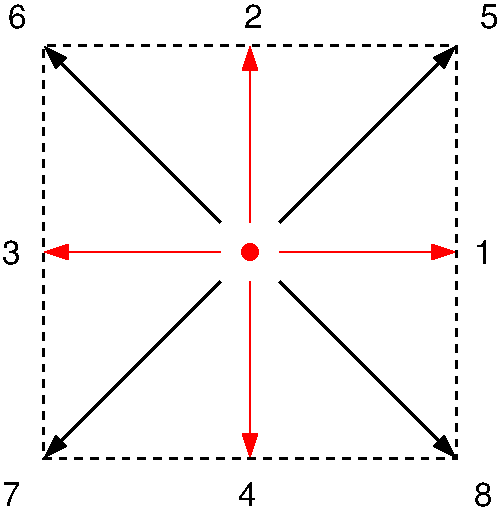
\includegraphics[width=\textwidth]{D2Q9.pdf}
\caption{D2Q5 (red) and D2Q9 (red and black) velocity directions. Direction 0 corresponds to the central node.}
\label{fig:d2q9}
\end{minipage}
\hspace{0.5cm}
\begin{minipage}[b]{0.475\linewidth}
\centering
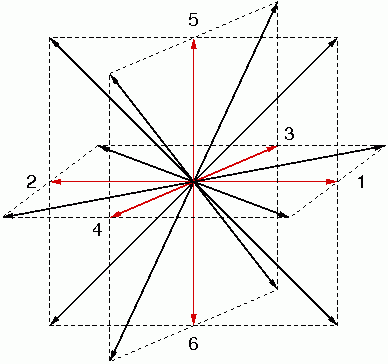
\includegraphics[width=\textwidth]{d3q19.png}
\caption{D3Q7 (red) and D3Q19 (read and black) velocity directions. Direction 0 corresponds to the central node.}
\label{fig:d3q19}
\end{minipage}
\end{figure}

\setlength{\tabcolsep}{4pt}
\begin{table}[h]\footnotesize
  \centering
\begin{tabular}{|c|r|r|r|r|r|r|r|}\hline
  % after \\: \hline or \cline{col1-col2} \cline{col3-col4} ...
  $i$      & 0 & 1 &  2 & 3 &  4 & 5 &  6\\\hline\hline
  $c_{ix}$ & 0 & 1 & -1 & 0 &  0 & 0 &  0\\
  $c_{iy}$ & 0 & 0 &  0 & 1 & -1 & 0 &  0\\
  $c_{iz}$ & 0 & 0 &  0 & 0 &  0 & 1 & -1\\\hline
\end{tabular}
 \caption{D3Q7 direction vectors}
\end{table}

\setlength{\tabcolsep}{4pt}
\begin{table}[h]\footnotesize
  \centering
\begin{tabular}{|c|r|r|r|r|r|r|r|r|r|r|r|r|r|r|r|r|r|r|r|}\hline
  % after \\: \hline or \cline{col1-col2} \cline{col3-col4} ...
  $i$      & 0 & 1 &  2 & 3 &  4 & 5 &  6 & 7 &  8 &  9 & 10 & 11 & 12 & 13 & 14 & 15 & 16 & 17 & 18 \\\hline\hline
  $c_{ix}$ & 0 & 1 & -1 & 0 &  0 & 0 &  0 & 1 & -1 &  1 & -1 &  1 & -1 &  1 & -1 &  0 &  0 &  0 &  0 \\
  $c_{iy}$ & 0 & 0 &  0 & 1 & -1 & 0 &  0 & 1 & -1 & -1 &  1 &  0 &  0 &  0 &  0 &  1 & -1 &  1 & -1 \\
  $c_{iz}$ & 0 & 0 &  0 & 0 &  0 & 1 & -1 & 0 &  0 &  0 &  0 &  1 & -1 & -1 &  1 &  1 & -1 & -1 &  1 \\\hline
\end{tabular}
 \caption{D3Q19 direction vectors}
\end{table}

\chapter{Implementation Details}
This chapter describes briefly the dual grid implementation as well as some practical implementation details.

\section{Dual Grid}
In the dual grid implementation two different grid resolutions are used for the momentum/pressure grid and the order parameter grid. Since all differential terms related to the interfacial force are calculated on the order parameter grid, a finer grid (twice as fine as the momentum/pressure grid) is used for the order parameter. Subsequently, two simulation steps are taken in the order parameter grid for simulation step in the momentum grid in order to maintain the data in the two grid in synchronization.

The velocity and the pressure are transferred from the momentum/pressure grid to the order parameter grid using bilinear interpolation, and all differential terms are calculated in the finer mesh and then copied over to the corresponding (overlapping) nodes in the momentum grid.

The advantage of using a dual grid implementation is that the results are nearly of the same quality than those obtained from a full refinement of both order parameter and momentum/pressure grid, but with considerable savings in computing time (~60\%) and memory use (~25\%).

\section{Interface Initialization}
The interface is initialized using the following profile in the direction normal ot the interface:

\begin{eqnarray}
\phi &=& \phi^*\tanh\left[\frac{2(r - R)}{W}\right] \quad\quad (ZSC-LBM)\\
\rho &=& \rho^*\tanh\left[\frac{2(r - R)}{W}\right] + \frac{1}{2}\left(\rho_{\rm L} + \rho_{\rm H}\right) \quad\quad (ZSC-LBM)
\end{eqnarray}

with $r$ the distance from any point in the fluid to the center a drop of radius $R$.

To be able to initialize several drops using this interface we only extend this between the center of the drop and $R+W$, so that any drops separated by more than $2W$ lattice units will be correctly initialized as individual units.

\section{Pressure Convergence}
A simple way to test when the relaxation of the interface between the two fluids has been achieved is to calculate teh deviation from Laplace's Law, which expresses the pressure difference between the inside and the inside of a drop as a function of the surface tension and the radius,

\begin{eqnarray}
P_{\rm in} - P_{\rm out} &=& \frac{\phantom{2}\sigma}{R} \quad\quad (2D)\;,\\
P_{\rm in} - P_{\rm out} &=& \frac{2\sigma}{R} \quad\quad (3D)\;.
\end{eqnarray}

In the code we calculate the relative pressure difference error as,

\begin{equation}
P_{\rm err} = (\delta P - \frac{\sigma}{R})\frac{R}{\sigma}\;,
\end{equation}

where $\delta P$ is the calculated pressure difference between the inside of the drop and the outside of the drop ignoring any values at the interface itself.

The error in the pressure difference is calculated every \verb+tStat+ iterations, and the difference between errors  calculated for consecutive iterations is stored in array \verb+Convergence+,

\begin{equation}
Convergence(i) = P_{\textrm{err},i} - P_{\textrm{err}, i-1}
\end{equation}

This calculation is done in function \verb+Stats+. After ten calls to \verb+Stats+ we calculate the average fluctuation in the pressure difference error by adding all the values in the array and dividing by ten,

\begin{equation}
\varepsilon = 0.1\sum_{i=1}^{10}{Convergence(i)}
\end{equation}

The relaxation run is stopped when this average fluctuation of the error is less than the given error limit \verb+pConv+.

\section{External Force}
The external force due to gravity is included via the E\"otv\"os number, a non-dimensional quantity that characterizes the  ratio of gravitational forces to interfacial forces and given by the expression:

\begin{equation}
Eo = \frac{g\left(\rho_H-\rho_L\right)D^2}{\sigma}
\end{equation}

Where $\sigma$ is the interface tension, $D$ is the characteristic bubble diameter and $\rho_H$ and $\rho_L$ anre the densities of the two fluids. In the code $Eo$ is taken as an input, and the acceleration corresponding to gravity in the lattice is obtained from this expression as:

\begin{equation}
g = \frac{\sigma Eo}{\left(\rho_H-\rho_L\right)D^2}
\end{equation}

The body force is expressed as $\vect{F_b}=(\rho_H-\rho_L)\vect{g}$ and introduced in the equations following the details in Section \ref{sec:zsc}.

\section{Optimized Version}
The optimized version of the code is based on the Zheng, Shu and Chew 3D model. The main differences with respect to the standard ZSC-3D version are:

\begin{itemize}
\item Change from Array of Structures (AOS) to Structure of Arrays (SOA)
	\begin{itemize}
	\item Each velocity direction has its own array
	\item Array indexing is in 1D using index $m=i+NX\cdot(j+NY\cdot k)+offset$
	\end{itemize}
\item OpenMP is used in the outermost loops
\item Added \verb+IVDEP+ directive to inner loops in \verb+collision+
\item Some rearrangement of operations inside \verb+collision+
\item No MPI
\item Simpler generation of file names (to be adopted in standard code soon)
\item All intermediate IO is controlled by pre-processor flags and can be eliminated
\end{itemize}

These changes improve performance in shared memory systems with wide vector units, and appear to be very effective in the Intel Xeon Phi coprocessors.

In the future two additional optimized version will be released a hybrid MPI/OpenMP version and a CUDA/MPI version. The standard implementations will always be provided for educational purposes.

\chapter{Benchmarking}
This section presents scaling results for the 3D versions of the code in the newest hardware available to the author. 

The first case we present is the scaling of a 240x480x480 domain calculation for the ZSC-3D-MPI code in the Stampede supercomputing cluster at TACC. Each compute node in Stampede consists of dual socket Intel Xeon E5-2680 "Sandy Bridge" processors and 32 GB of RAM, as well as an Intel Xeon Phi SE10P coprocessor  with 8GB of memory. Nodes are connected with  Mellanox FDR Infiniband in a two-level (core/leaf) fat tree setup. The compiler used was Intel 13.1, the MPI library used was Mvapich2 v1.9a2, and the compilation flags for this test case were simply \verb+-O3 -xAVX+. Results for scaling are shown in Figure \ref{fig:scaling_mpi} in terms of MLUPS (millions of lattice updates per second).

\begin{figure}[!htb]
\centering
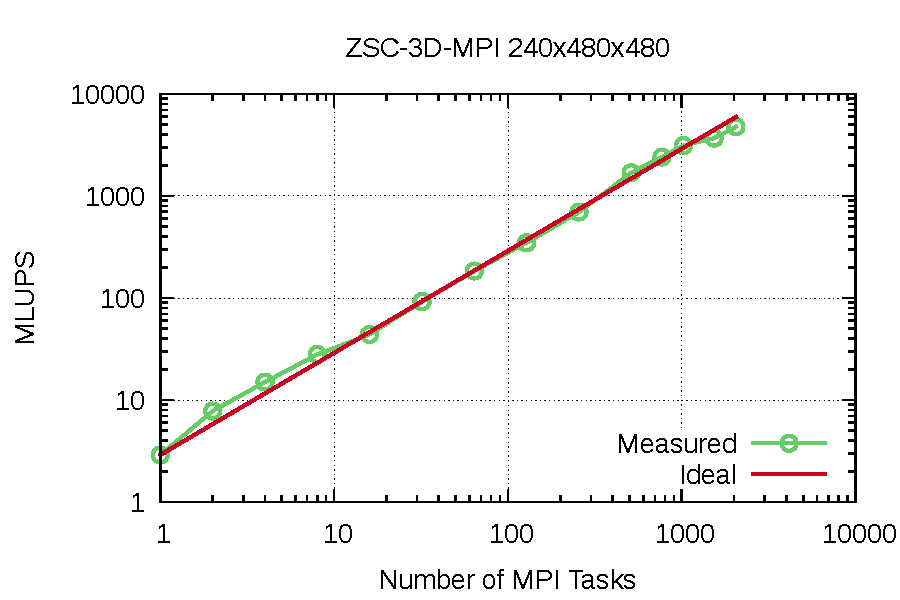
\includegraphics[width=0.7\textwidth]{scaling_mpi.pdf}
\caption{Scaling of standard \texttt{ZSC-3D-MPI} code.}
\label{fig:scaling_mpi}
\end{figure}

\begin{figure}[!htb]
\centering
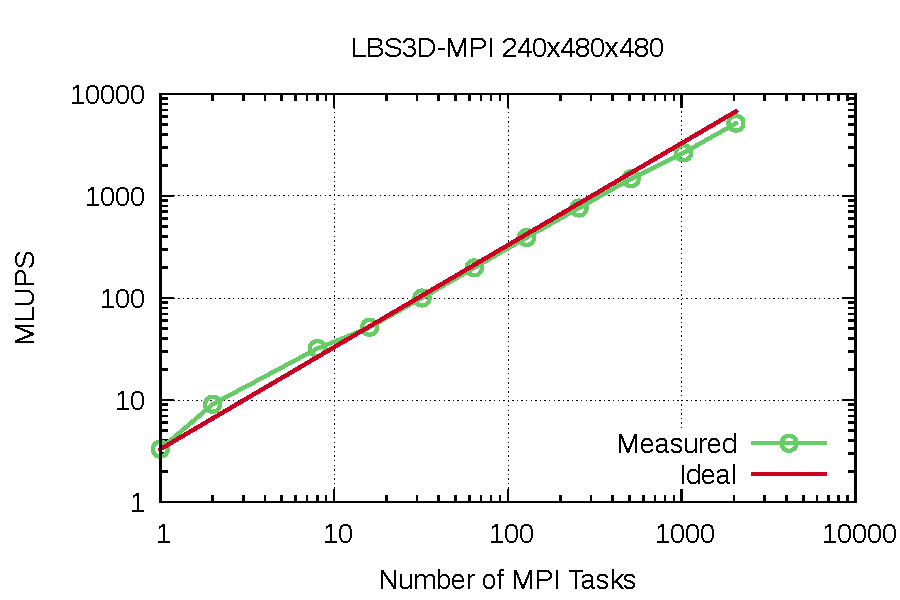
\includegraphics[width=0.7\textwidth]{scaling_hybrid.pdf}
\caption{Scaling of hybrid \texttt{LBS3D-MPI} code.}
\label{fig:scaling_hybrid}
\end{figure}

The benchmark shows that the scalability of the code is high, with the Zheng-Shu-Chew model maintaining 80\% parallel efficiency even at 2048 tasks, when each task is only processing a total of 27,000 grid points. A similar behavior is shown by the LBS3D-MPI code -- Figure \ref{fig:scaling_hybrid} -- that when using 2 tasks per node and 8 threads per task achieves a parallel efficiency of over 76\% at 2048 cores, and has a throughput that is 8\% higher than that of the less optimized ZSC-3D-MPI code.

The optimized \verb+LBS3D+ code has been benchmarked on TACC's Stampede and Lonestar Linux clusters. Each compute node on Stampede consists of dual socket Intel Xeon E5-2680 "Sandy Bridge" processors and 32 GB of RAM, as well as an Intel Xeon Phi SE10P with 8GB of memory. Each compute node in Lonestar consists of dual socket Intel Xeon X5680 "Westmere" processors and 24 GB or RAM. In the case of Lonestar the Intel compiler v11.1 and the Mvapich2 1.6 library were used.

The test case used was a 240x240x240 domain, and the the results are shown in Figure \ref{fig:scaling_cpu} below.

\begin{figure}[!htb]
\centering
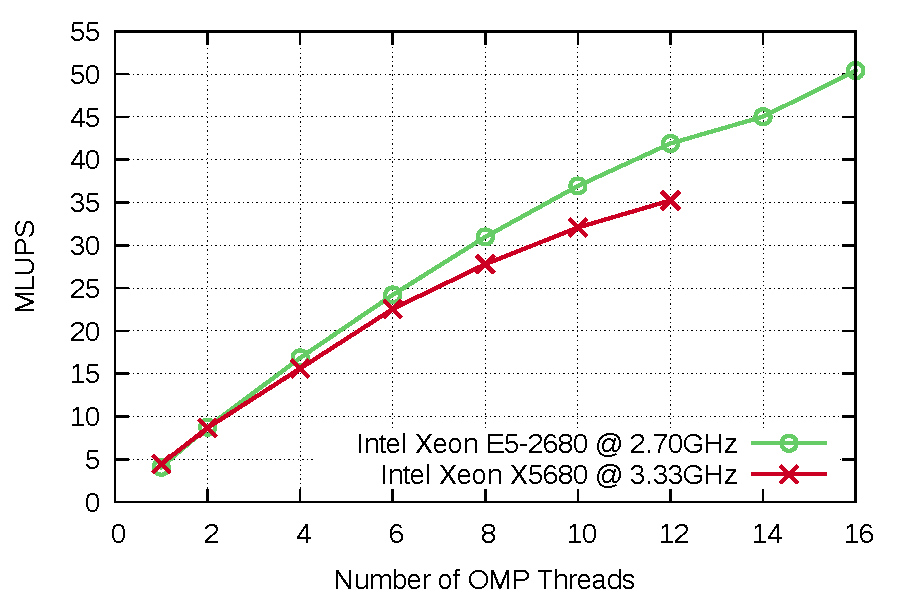
\includegraphics[width=0.7\textwidth]{scaling_cpu.pdf}
\caption{Speedup test for LBS3D on two Linux systems.}
\label{fig:scaling_cpu}
\end{figure}

Tests run on the Intel Xeon Phi coprocessor used the \verb+-openmp -O3 -mmic+ compilation flags, and thread binding was specified using the environmental variable \verb+KMP_AFFINITY=balanced,granularity=fine+. The results are shown in Figure \ref{fig:scaling_mic}. The rate of performance increase drops when more than one thread per core is used, although the code continues getting faster until all possible threads in the system are in use. Note that the maximum performance achieve on the Xeon Phi coprocessor is more than 2X the maximum performance achieve on two sockets of a regular E5-2680 CPU.

\begin{figure}[!htb]
\centering
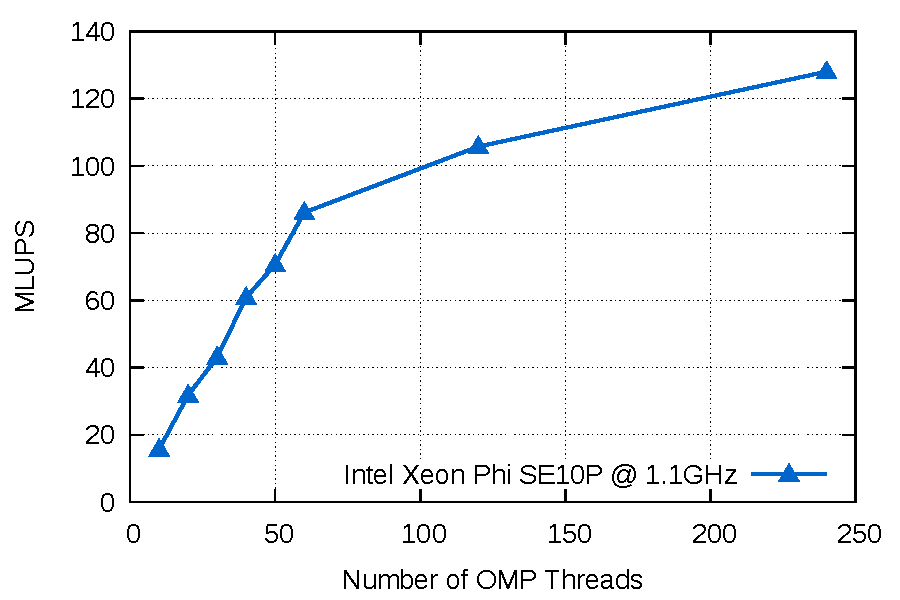
\includegraphics[width=0.7\textwidth]{scaling_mic.pdf}
\caption{Speedup test for LBS3D on the Intel Xeon Phi platform.}
\label{fig:scaling_mic}
\end{figure}

\chapter{Subroutine Listing}

\vspace{-1em}
\fcolorbox{black}{LightGrey}{
\begin{tabular}{ll}
Directory&: \texttt{mplabs/src/devel/offload}\\
Source Files&: 25
\end{tabular}}

\begin{verbatim}
collision.F90     packcpu.F90           relaxstats.F90
collisionmic.F90  packcpu_f.F90         stats.F90
common.F90        packmic.F90           stream.F90
finalsave.F90     packmic_f.F90         streammic.F90
init.F90          parameters.F90        updatephi.F90
initmic.F90       postcollision.F90     updatephimic.F90
main.F90          postcollisionmic.F90  vtksave.F90
Makefile          poststream.F90
memalloc.F90      poststreammic.F90
\end{verbatim}
\hrule\vspace{1em}


\vspace{-1em}
\fcolorbox{black}{LightGrey}{
\begin{tabular}{ll}
Directory&: \texttt{mplabs/src/devel/omp\_v1}\\
Source Files&: 14
\end{tabular}}

\begin{verbatim}
collision.F90  Makefile           relaxstats.F90
common.F90     memalloc.F90       stats.F90
finalsave.F90  parameters.F90     stream.F90
init.F90       postcollision.F90  vtksave.F90
main.F90       poststream.F90
\end{verbatim}
\hrule\vspace{1em}

\vspace{-1em}
\fcolorbox{black}{LightGrey}{
\begin{tabular}{ll}
Directory&: \texttt{mplabs/src/devel/omp\_v2}\\
Source Files&: 14
\end{tabular}}

\begin{verbatim}
collision.F90  Makefile           relaxstats.F90
common.F90     memalloc.F90       stats.F90
finalsave.F90  parameters.F90     stream.F90
init.F90       postcollision.F90  vtksave.F90
main.F90       poststream.F90
\end{verbatim}
\hrule\vspace{1em}

\vspace{-1em}
\fcolorbox{black}{LightGrey}{
\begin{tabular}{ll}
Directory&: \texttt{mplabs/src/devel/sequential}\\
Source Files&: 14
\end{tabular}}

\begin{verbatim}
collision.F90  Makefile           relaxstats.F90
common.F90     memalloc.F90       stats.F90
finalsave.F90  parameters.F90     stream.F90
init.F90       postcollision.F90  vtksave.F90
main.F90       poststream.F90
\end{verbatim}
\hrule\vspace{1em}

\vspace{-1em}
\fcolorbox{black}{LightGrey}{
\begin{tabular}{ll}
Directory&: \texttt{mplabs/src/devel/soa}\\
Source Files&: 14
\end{tabular}}

\begin{verbatim}
collision.F90  Makefile           relaxstats.F90
common.F90     memalloc.F90       stats.F90
finalsave.F90  parameters.F90     stream.F90
init.F90       postcollision.F90  vtksave.F90
main.F90       poststream.F90
\end{verbatim}
\hrule\vspace{1em}

\vspace{-1em}
\fcolorbox{black}{LightGrey}{
\begin{tabular}{ll}
Directory&: \texttt{mplabs/src/devel/soa\_aligned}\\
Source Files&: 14
\end{tabular}}

\begin{verbatim}
collision.F90  Makefile           relaxstats.F90
common.F90     memalloc.F90       stats.F90
finalsave.F90  parameters.F90     stream.F90
init.F90       postcollision.F90  vtksave.F90
main.F90       poststream.F90
\end{verbatim}
\hrule\vspace{1em}

\vspace{-1em}
\fcolorbox{black}{LightGrey}{
\begin{tabular}{ll}
Directory&: \texttt{mplabs/src/opt/lbs3d}\\
Source Files&: 14
\end{tabular}}

\begin{verbatim}
collision.F90  Makefile           relaxstats.F90
common.F90     memalloc.F90       stats.F90
finalsave.F90  parameters.F90     stream.F90
init.F90       postcollision.F90  vtksave.F90
main.F90       poststream.F90
\end{verbatim}
\hrule\vspace{1em}

\vspace{-1em}
\fcolorbox{black}{LightGrey}{
\begin{tabular}{ll}
Directory&: \texttt{mplabs/src/opt/lbs3d-mpi}\\
Source Files&: 15
\end{tabular}}

\begin{verbatim}
collision.F90  Makefile           relaxstats.F90
common.F90     memalloc.F90       stats.F90
finalsave.F90  parameters.F90     stream.F90
init.F90       postcollision.F90  vgrid.F90
main.F90       poststream.F90     vtksave.F90
\end{verbatim}
\hrule\vspace{1em}

\vspace{-1em}
\fcolorbox{black}{LightGrey}{
\begin{tabular}{ll}
Directory&: \texttt{mplabs/src/std/ll-dgr-mpi}\\
Source Files&: 23
\end{tabular}}

\begin{verbatim}
common.f           mpi_update_f.f      prestream_f.f
finaldump.f        mpi_update_g.f      prestream_g.f
hydrodynamics_f.f  mpi_update_hydro.f  stats.f
hydrodynamics_g.f  mpi_update_rho_f.f  update_f.f
init.f             mpi_update_rho_g.f  update_g.f
main.f             parameters.f        vgrid.f
Makefile           poststream_f.f      vtkplane.f
memalloc.f         poststream_g.f
\end{verbatim}
\hrule\vspace{1em}

\fcolorbox{black}{LightGrey}{
\begin{tabular}{ll}
Directory&: \texttt{mplabs/src/std/ll-dgr-seq}\\
Source Files&: 17
\end{tabular}}

\begin{verbatim}
common.F90           Makefile          prestream_g.F90
finaldump.F90        memalloc.F90      stats.F90
hydrodynamics_f.F90  parameters.F90    update_f.F90
hydrodynamics_g.F90  poststream_f.F90  update_g.F90
init.F90             poststream_g.F90  vtkplane.F90
main.F90             prestream_f.F90
\end{verbatim}
\hrule\vspace{1em}

\fcolorbox{black}{LightGrey}{
\begin{tabular}{ll}
Directory&: \texttt{mplabs/src/std/ll-mpi}\\
Source Files&: 15
\end{tabular}}

\begin{verbatim}
common.f         Makefile         poststream.f
finaldump.f      memalloc.f       prestream.f
hydrodynamics.f  mpi_updatefg.f   stats.f
init.f           mpi_updaterho.f  vgrid.f
main.f           parameters.f     vtkplane.f
\end{verbatim}
\hrule\vspace{1em}

\fcolorbox{black}{LightGrey}{
\begin{tabular}{ll}
Directory&: \texttt{mplabs/src/std/ll-seq}\\
Source Files&: 12
\end{tabular}}

\begin{verbatim}
common.F90         main.F90        poststream.F90
finaldump.F90      Makefile        prestream.F90
hydrodynamics.F90  memalloc.F90    stats.F90
init.F90           parameters.F90  vtkplane.F90
\end{verbatim}
\hrule\vspace{1em}

\fcolorbox{black}{LightGrey}{
\begin{tabular}{ll}
Directory&: \texttt{mplabs/src/std/zsc-3d-mpi}\\
Source Files&: 16
\end{tabular}}

\begin{verbatim}
collision.f       Makefile         stats.f
collisionrelax.f  memalloc.f       stream.f
common.f          parameters.f     vgrid.f
finaldump.f       postcollision.f  vtkdump.f
init.f            poststream.f
main.f            relaxstats.f
\end{verbatim}
\hrule\vspace{1em}

\fcolorbox{black}{LightGrey}{
\begin{tabular}{ll}
Directory&: \texttt{mplabs/src/std/zsc-dgr-mpi}\\
Source Files&: 18
\end{tabular}}

\begin{verbatim}
collision_f.f    main.f             poststream_f.f
collision_g.f    Makefile           stats.f
common.f         memalloc.f         stream.f
differentials.f  parameters.f       update.f
finaldump.f      postcollision_f.f  vgrid.f
init.f           postcollision_g.f  vtkplane.f
\end{verbatim}
\hrule\vspace{1em}

\fcolorbox{black}{LightGrey}{
\begin{tabular}{ll}
Directory&: \texttt{mplabs/src/std/zsc-dgr-seq}\\
Source Files&: 14
\end{tabular}}

\begin{verbatim}
collision_f.F90    init.F90        stats.F90
collision_g.F90    main.F90        stream.F90
common.F90         Makefile        update.F90
differentials.F90  memalloc.F90    vtkplane.F90
finaldump.F90      parameters.F90
\end{verbatim}
\hrule\vspace{1em}
\pagebreak

\fcolorbox{black}{LightGrey}{
\begin{tabular}{ll}
Directory&: \texttt{mplabs/src/std/zsc-seq}\\
Source Files&: 14
\end{tabular}}

\begin{verbatim}
collision.f  Makefile         stats.f
common.f     memalloc.f       stream.f
finaldump.f  parameters.f     vgrid.f
init.f       postcollision.f  vtkplane.f
main.f       poststream.f
\end{verbatim}
\hrule\vspace{1em}
\pagebreak

\fcolorbox{black}{LightGrey}{
\begin{tabular}{ll}
Directory&: \texttt{mplabs/src/std/zsc-seq}\\
Source Files&: 14
\end{tabular}}

\begin{verbatim}
collision.f  Makefile            stats.f
common.f     memalloc.f          stream.f
finaldump.f  mplabs_install.err  vtkplane.f
init.f       mplabs_install.log
main.f       parameters.f
\end{verbatim}
\hrule\vspace{1em}

\pagebreak
\section*{}
\pagebreak

\addcontentsline{toc}{chapter}{References}
\begin{thebibliography}{00}

\bibitem{gnuplot} Gnuplot is a command-line driven interactive data and function plotting utility distributed as copyrighted but free software. For more information visit the official Gnuplot web site \verb+http://www.gnuplot.info/+.

\bibitem{paraview} Paraview is an open source multi-platform visualization application	that provides options relevant to the scientific community such as	parallel rendering facilities for large data sets. For more information visit the official web site at \verb+http://www.paraview.org/+.

\bibitem{Rosales2013} C. Rosales,  Porting to the Intel Xeon Phi: Opportunities and Challenges. Extreme Scaling Workshop 2013 (XSCALE13), Boulder, CO, USA (2013).

\bibitem{Rosales2007} C. Rosales, D.S. Whyte and M. Cheng, A massively parallel Lattice Boltzmann Method for large density ratios, Proceedings of the 7th Asian CFD Conference, Bangalore, India, 1371 (2007)

\bibitem{Rosales2010} C. Rosales and D. S. Whyte, Dual Grid Lattice Boltzmann Method for Multiphase Flows. {\it International Journal for Numerical Methods in Engineering} 84: 1068--1084 (2010).

\bibitem{openmpi} The Open MPI project is an open source MPI-2 implementation developed and maintained by a consortium of academic, research, and industry partners. Learn more at \verb+http://www.open-mpi.org/+.

\bibitem{Zheng2006} H.W. Zheng, C. Shu and Y.T. Chew, A lattice Boltzmann model for multiphase flows with large density ratio, J. Comput. Phys. 218, 353 (2006)

\bibitem{Lee2005} T. Lee and C.-L. Lin, A stable discretization of the lattice Boltzmann equation for simulation of incompressible two-phase flows at high density ratio, J. Comput. Phys. 206, 16 (2005)

\bibitem{Bhatnagar1954} P.L. Bhatnagar, E.P. Gross and M. Krook, A model for collision processes in gases. I. Small amplitude processes in charged and neutral one-component systems, Phys. Rev. 94, 511 (1954)

\end{thebibliography}

\end{document}
